\documentclass[11pt,compress,t,notes=noshow, aspectratio=169, xcolor=table]{beamer}

\usepackage{../../style/lmu-lecture}

% %  New colors
\definecolor{ggRed}{HTML}{F8766D}
\definecolor{ggGreen}{HTML}{00BFC4}
\definecolor{rep}{HTML}{3646f1}
\definecolor{cice}{HTML}{00BFFF}

% Defines macros and environments
% This file is included in slides and exercises

% Rarely used fontstyle for R packages, used only in 
% - forests/slides-forests-benchmark.tex
% - exercises/single-exercises/methods_l_1.Rnw
% - slides/cart/attic/slides_extra_trees.Rnw
\newcommand{\pkg}[1]{{\fontseries{b}\selectfont #1}}

% Spacing helpers, used often (mostly in exercises for \dlz)
\newcommand{\lz}{\vspace{0.5cm}} % vertical space (used often in slides)
\newcommand{\dlz}{\vspace{1cm}}  % double vertical space (used often in exercises, never in slides)
\newcommand{\oneliner}[1] % Oneliner for important statements, used e.g. in iml, algods
{\begin{block}{}\begin{center}\begin{Large}#1\end{Large}\end{center}\end{block}}

% Don't know if this is used or needed, remove?
% textcolor that works in mathmode
% https://tex.stackexchange.com/a/261480
% Used e.g. in forests/slides-forests-bagging.tex
% [...] \textcolor{blue}{\tfrac{1}{M}\sum^M_{m} [...]
% \makeatletter
% \renewcommand*{\@textcolor}[3]{%
%   \protect\leavevmode
%   \begingroup
%     \color#1{#2}#3%
%   \endgroup
% }
% \makeatother


\title{Interpretable Machine Learning}
% \author{LMU}
%\institute{\href{https://compstat-lmu.github.io/lecture_iml/}{compstat-lmu.github.io/lecture\_iml}}
\date{}

\begin{document}

\newcommand{\titlefigure}{figure/ale_plot.pdf}
\newcommand{\learninggoals}{
\item Difference between feature effects and feature interactions
\item REPID
\item GADGET
}

\lecturechapter{Regional Effects}
\lecture{Interpretable Machine Learning}

\begin{frame}{REPID: Regional Effect Plots \citebutton{Herbinger et al. (2022)}{https://proceedings.mlr.press/v151/herbinger22a.html}}

\textbf{Recall:} Different shapes of ICE curves indicate interactions (we want to ignore vertical shifts)\\
$\Rightarrow$ Focus on shape differences of {\color{cice}\bfseries mean-centered ICE curves}.
    
%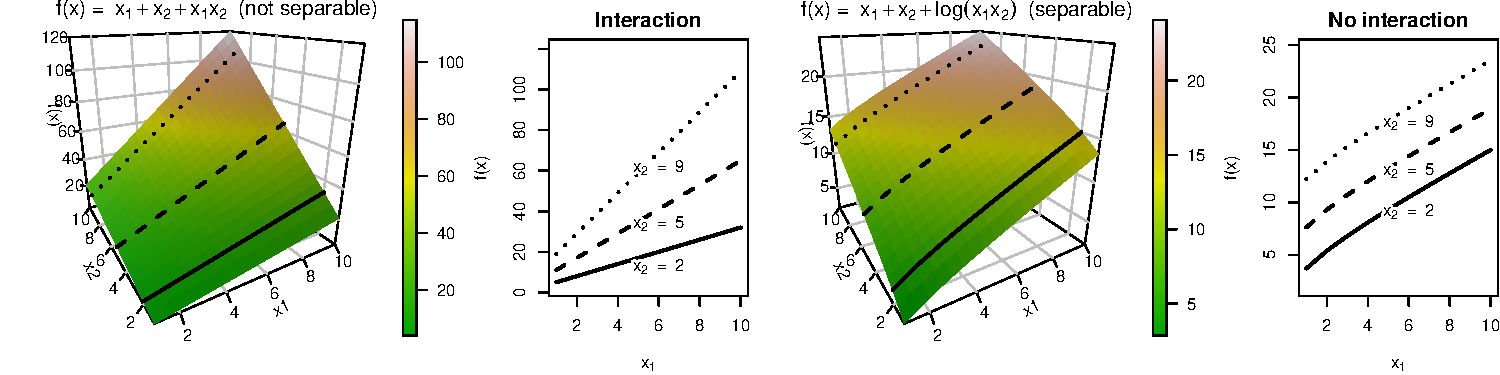
\includegraphics[width = 0.8\textwidth, trim={0cm 0cm 0cm 0cm}, clip]{figure/interaction_separable_2}

The mean-centered ICE curve for obs. $\xv$ evaluated at $m$ grid points $\tilde x_j^{(1)}, \dots, \tilde x_j^{(m)}$ is:

{\color{cice}
\centerline{$\hat f^c(\tilde x_j, \xv_{-j}) = \hat{f}(\tilde x_j, \xv_{-j}) - \frac{1}{m} \sum\nolimits_{k=1}^m \hat{f}(\tilde x_j^{(k)}, \xv_{-j})$}}
 %and $g \in \{1,...,G\}$

\begin{columns}
    \begin{column}{0.39\textwidth}
        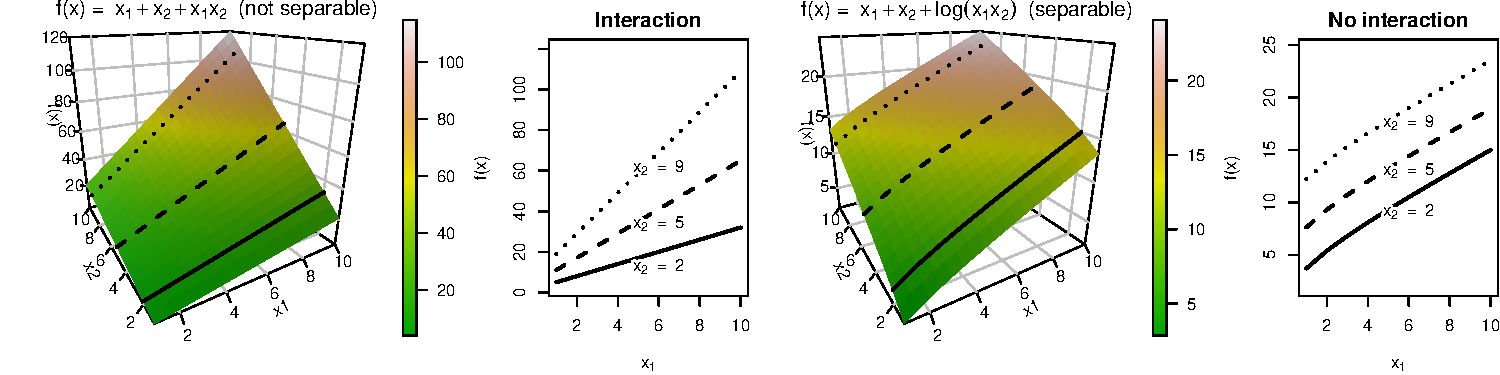
\includegraphics[width = \textwidth, trim={13cm 0cm 0cm 0cm}, clip]{figure/interaction_separable_2}
    \end{column}
    \begin{column}{0.61\textwidth}
        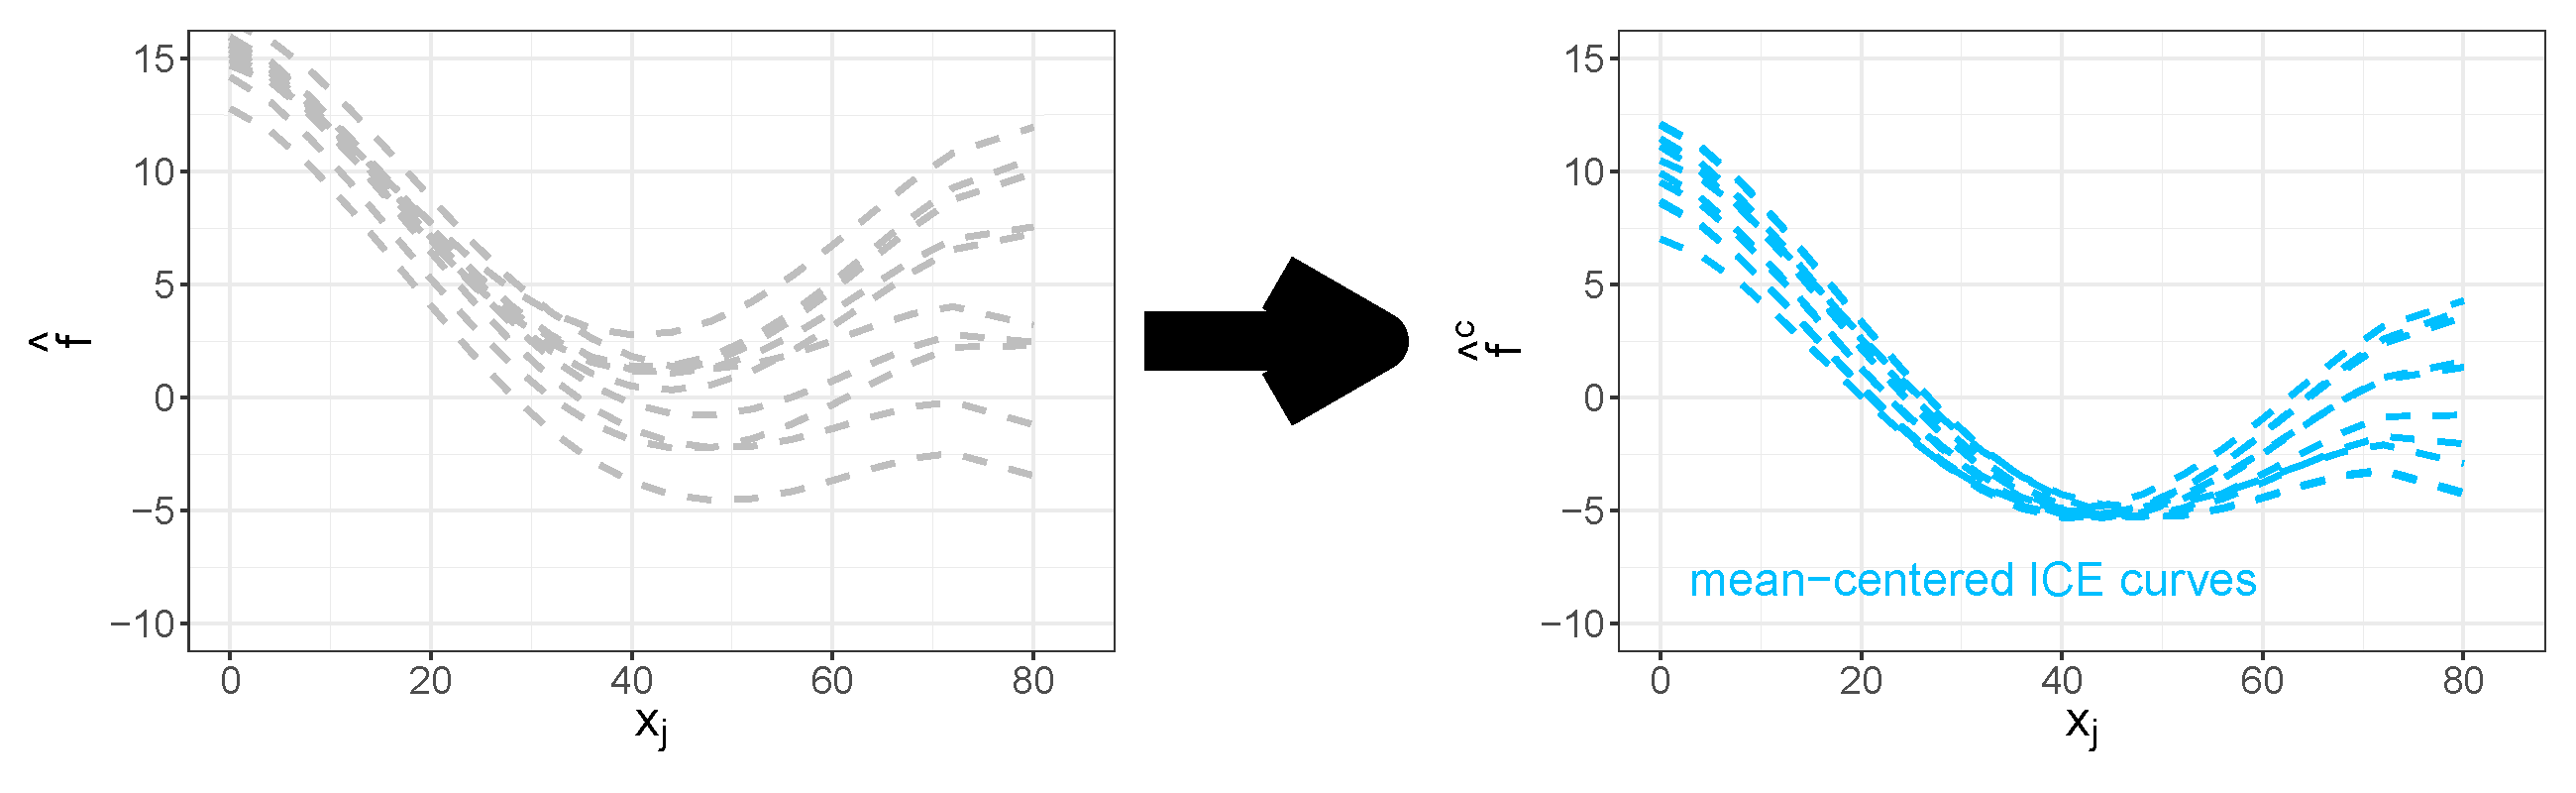
\includegraphics[width = \textwidth]{figure/ice_rep_distance0.png} 
    \end{column}
\end{columns}

%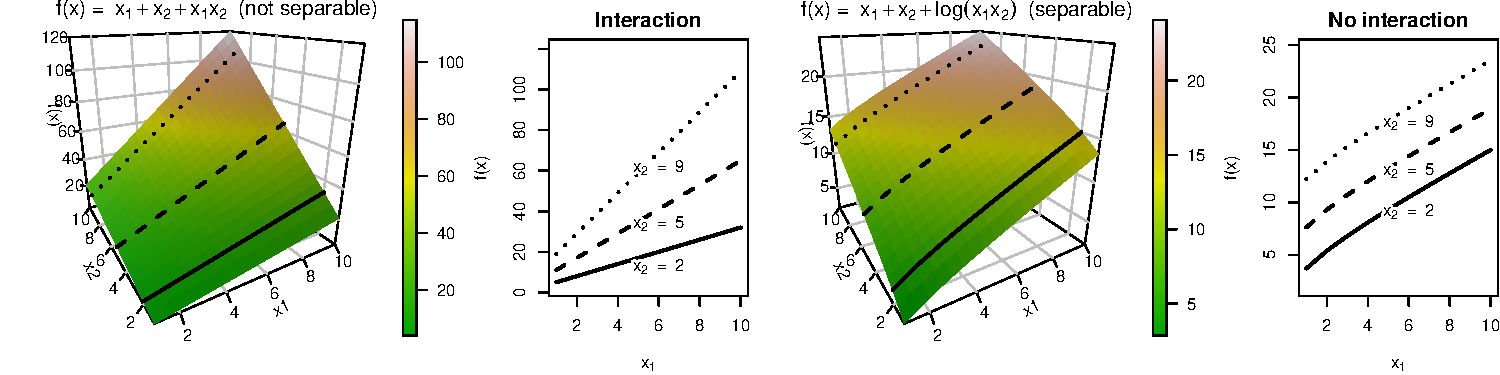
\includegraphics[width = 0.3\textwidth, trim={13cm 0cm 0cm 0cm}, clip]{figure/interaction_separable_2}
\end{frame}

\begin{frame}{Regional Effect Plots - Intuition}

\begin{columns}[T, totalwidth=\textwidth]
    \begin{column}{0.6\textwidth}
 Define risk as the L2 loss of mean-centered ICE curves:
$$\textstyle
    \mathcal{R}\left(\mathcal{N}\right) =
    \sum\limits_{\xv \in \mathcal{N}} 
     \sum\limits_{k = 1}^m
     (\underbrace{{\color{cice}\hat f^{c}(\tilde x_j^{(k)}, \xv_{-j})} - \color{rep}\hat f_{j|\mathcal{N}}^{PD,c} (\tilde x_j^{(k)})}_\text{$\color{orange}{d_k}$})^2
    %\mathcal{L}\left(\xv_j, i\right)
    $$
with the average feature effect in %region with associated index set 
region $\mathcal{N} \subseteq \Xspace$:

\medskip

{\color{rep}
\centerline{$ \displaystyle    \hat f_{j|\mathcal{N}}^{PD,c}(\tilde x_j) = \frac{1}{|\mathcal{N}|} \sum_{\xv \in \mathcal{N}} \hat f^c(\tilde x_j, \xv_{-j})$}}
    \end{column}
    \begin{column}{0.39\textwidth}
            \centering
    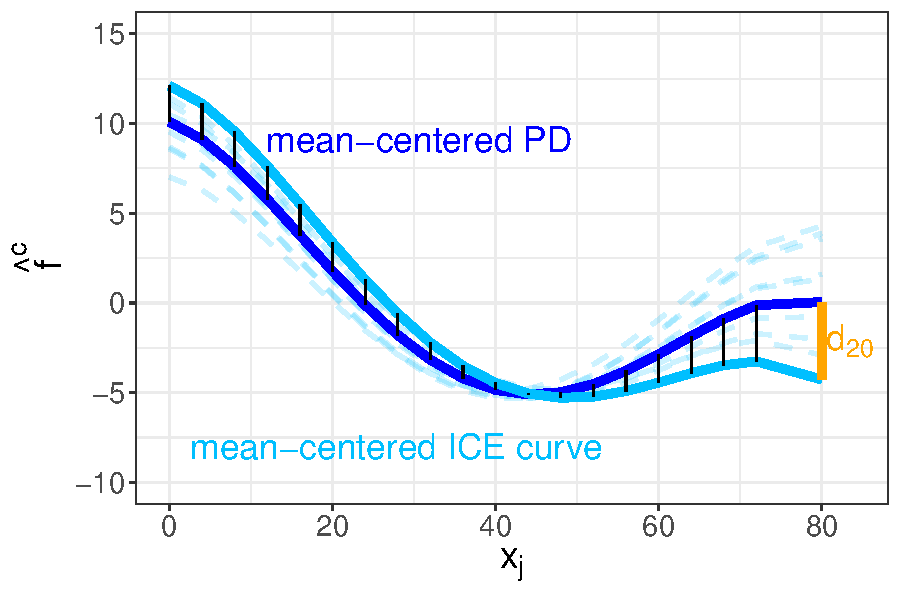
\includegraphics[width = \textwidth]{figure/ice_rep_distance2.pdf}
    \end{column}
\end{columns}
%\medskip
\begin{itemize}
    \item[$\Rightarrow$] Measures interaction-related heterogeneity (variance) ICE curves in region $\mathcal{N}$
    \item[$\Rightarrow$] Recursive partitioning (as in CART): Find the best feature-split combination that minimizes
    
\medskip

\centerline{$\mathcal{R}\left(\mathcal{N}_{left}\right) + \mathcal{R}\left(\mathcal{N}_{right}\right)$}
\end{itemize}

      \begin{columns}[c, totalwidth=\textwidth]
        \begin{column}{0.4\textwidth}
    \begin{itemize}
        \item $\mathcal{N}_{left} = \{\xv \in \mathcal{N}|x_z \leq t\}$
        \item $\mathcal{N}_{right} = \{\xv \in \mathcal{N}|x_z > t\}$
        \item Split point $t$ for feature $x_z, z \in -j$
    \end{itemize}
        \end{column}
          \begin{column}{0.59\textwidth}
          \centering
          \textbf{Intuition:} Is another feature $x_z$ \\responsible for the heterogeneity?
        \end{column}
    \end{columns}
        %\item loss $\mathcal{L}$ for $i$-th ICE curve based on a grid of size $m$
        %\item aggregate over all ICEs within region $\mathcal{N}$
    %\end{itemize}
%\footnote[frame]{\textbf{AISTATS 2022:} \textit{REPID - Regional Effect Plots with implicit Interaction Detection}}
\end{frame}

\begin{frame}{Regional Effect Plots - Example}

   
%\textbf{How can we use ICE curves to find regions with representative PDPs?}
%\vspace*{0.3cm}

\begin{columns}[T, totalwidth = \linewidth]
    \begin{column}{0.42\textwidth}


\textbf{Example:}
%$X_1, X_2 \sim \mathcal{U}(-1,1), X_3, X_5 \sim \mathcal{B}(n, 0.5), X_4 \sim \mathcal{B}(n, 0.7), X_6 \sim \mathcal{N}(1,5)$ (all iid)\\
$X_1, X_2, X_6 \sim \mathcal{U}(-1,1)$, 
$X_3, X_4, X_5 \sim \mathcal{B}(n, 0.5)$ (all iid)\\

%$\leadsto$ True relationship: $f(X) = 0.2 X_1 - 8 X_2 + \color{YellowGreen}{8 X_2  \mathbbm{1}_{(X_1 > 0)}} \color{black}+ \color{ForestGreen}{16 X_2  \mathbbm{1}_{(X_3 = 0)}} \color{black}+ \epsilon, \; \epsilon \sim \mathcal{N}(0,1)$\\

$\leadsto$ Model: Random forest

        \begin{itemize}
  %\setlength{\itemindent}{0em}
\item \textbf{Problem:} 
\begin{itemize}
    \item \only<1>{PD curve of ${X_2}$ is misleading due to interactions $\leadsto$ ICE}
    \only<2->{PD curve of $X_2$ is misleading due to interactions $\leadsto$ ICE}
    \item ICE curves do not identify the interacting features
\end{itemize}

\item<2-> \textbf{Idea:} Find regions where variance of ICE curves is minimized by recursive partitioning the feature space w.r.t. all other features $-j$\\
%Find regions with similar ICE curves and aggregate them to regional effects\\
%\item 
%$\leadsto$ REP more representative due to less interactions  
   %\item[$\leadsto$]\textbf{Idea} Recursively partition feature space w.r.t. $-j$ such that distance of ICE curves to REP is small}
\item<3-> {\color{rep}\textbf{Regional effect}} (blue curves)   $\hat = $ Estimate PD curve in each region

 % \centerline{$ \textstyle    \hat f_{j|\mathcal{N}_g}^{PD}(\tilde x_j) = \frac{1}{|\mathcal{N}_g|} \sum_{i \in \mathcal{N}_g} \hat f(\tilde x_j, \xv_{-j}^{(i)})$}
\end{itemize}


   
    \end{column}
    \begin{column}{0.55\textwidth}
    \small
    \only<1>{\centerline{
    $f(X) = 0.2 X_1 {- 8 X_2 + {8 X_2  \mathbbm{1}_{(X_1 > 0)}}+ {16 X_2  \mathbbm{1}_{(X_3 = 0)}}} + \epsilon $}}
    \only<2>{\centerline{
    $f(X) = 0.2 X_1 - 8 X_2 + {8 X_2  \mathbbm{1}_{(X_1 > 0)}} + FG{16 X_2  \mathbbm{1}_{(X_3 = 0)}} \color{black}+ \epsilon $}}
    \only<3>{\centerline{
    $f(X) = 0.2 X_1 - 8 X_2 + YG{8 X_2  \mathbbm{1}_{(X_1 > 0)}} \color{black}+ FG{16 X_2  \mathbbm{1}_{(X_3 = 0)}} \color{black}+ \epsilon $}}
    %$, \; \epsilon \sim \mathcal{N}(0,1)$
\only<1>{
    \centering
      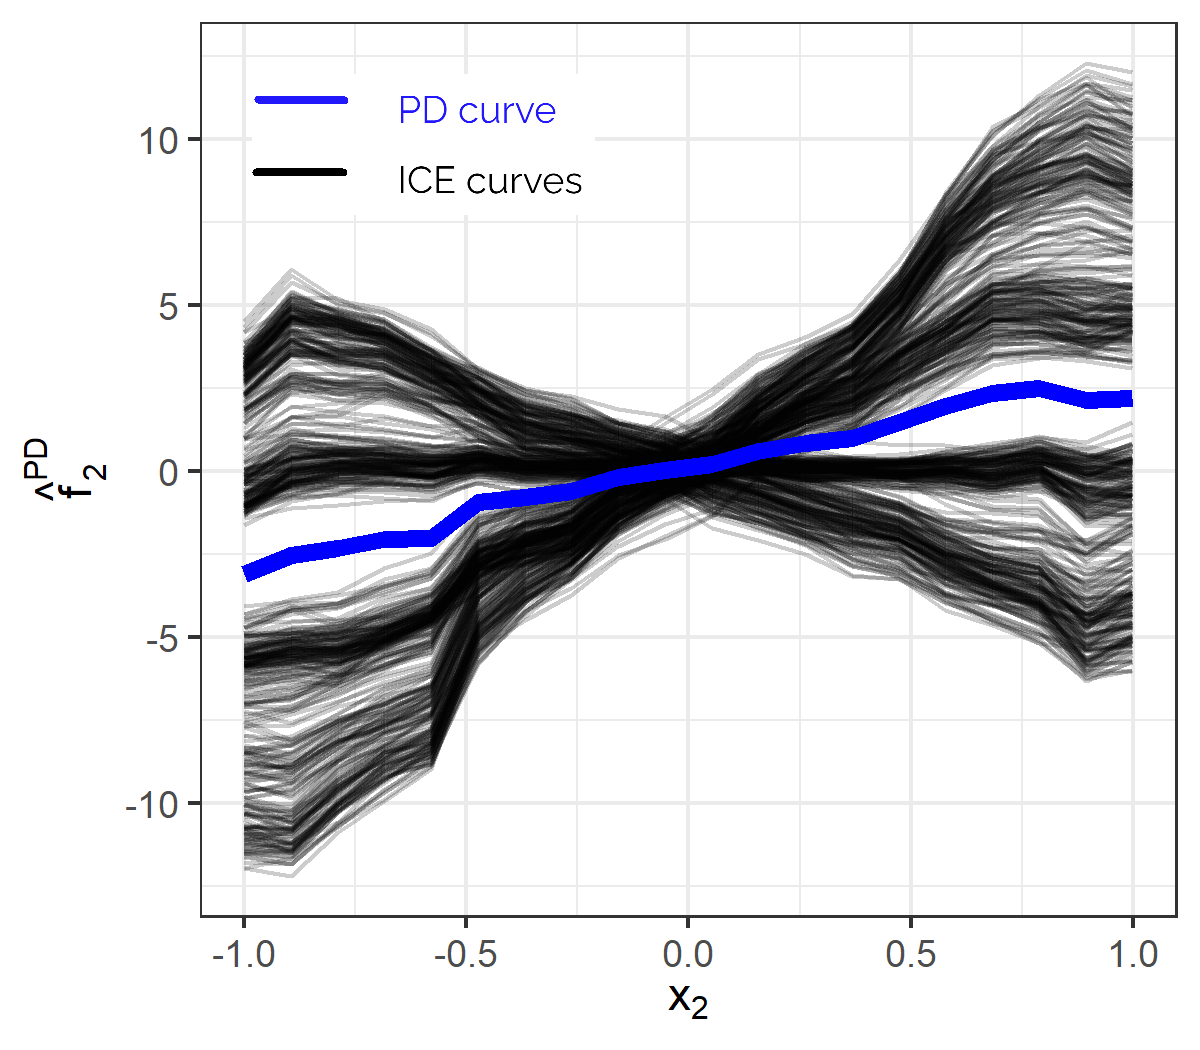
\includegraphics[width=0.82\textwidth]{figure/sim1_allcurves.png} 
}
\only<2->{
\centering
     %\begin{minipage}[t]{.5\textwidth}
     \hspace{-20pt}
     \includegraphics<2>[width=0.5\textwidth]{figure/sim1_allcurves.png}
     
     \only<2>{
           \begin{tikzpicture}
      \usetikzlibrary{arrows}
        \usetikzlibrary{shapes}
         \tikzset{treenode/.style={draw}}
         \tikzset{line/.style={draw, thick}}
     % Nodes
    \node [treenode] (a0) {}; [below=1pt,at=(10,0)]  {};% Top node
    \node [treenode, below=0.3cm of a0, xshift=-1.0cm] (a1) {}; % Bottom left node
    \node [treenode, below=0.3cm of a0, xshift=1.0cm] (a2) {}; % Bottom right node

    % Lines
    \draw [thick] (a0) -- ++(0, -0.2cm) -| (a1);
    \draw [thick] (a0) -- ++(0, -0.2cm) -| (a2);
      \end{tikzpicture}
     }
     
      %\fcolorbox{ForestGreen}{white}     {
      FG{
      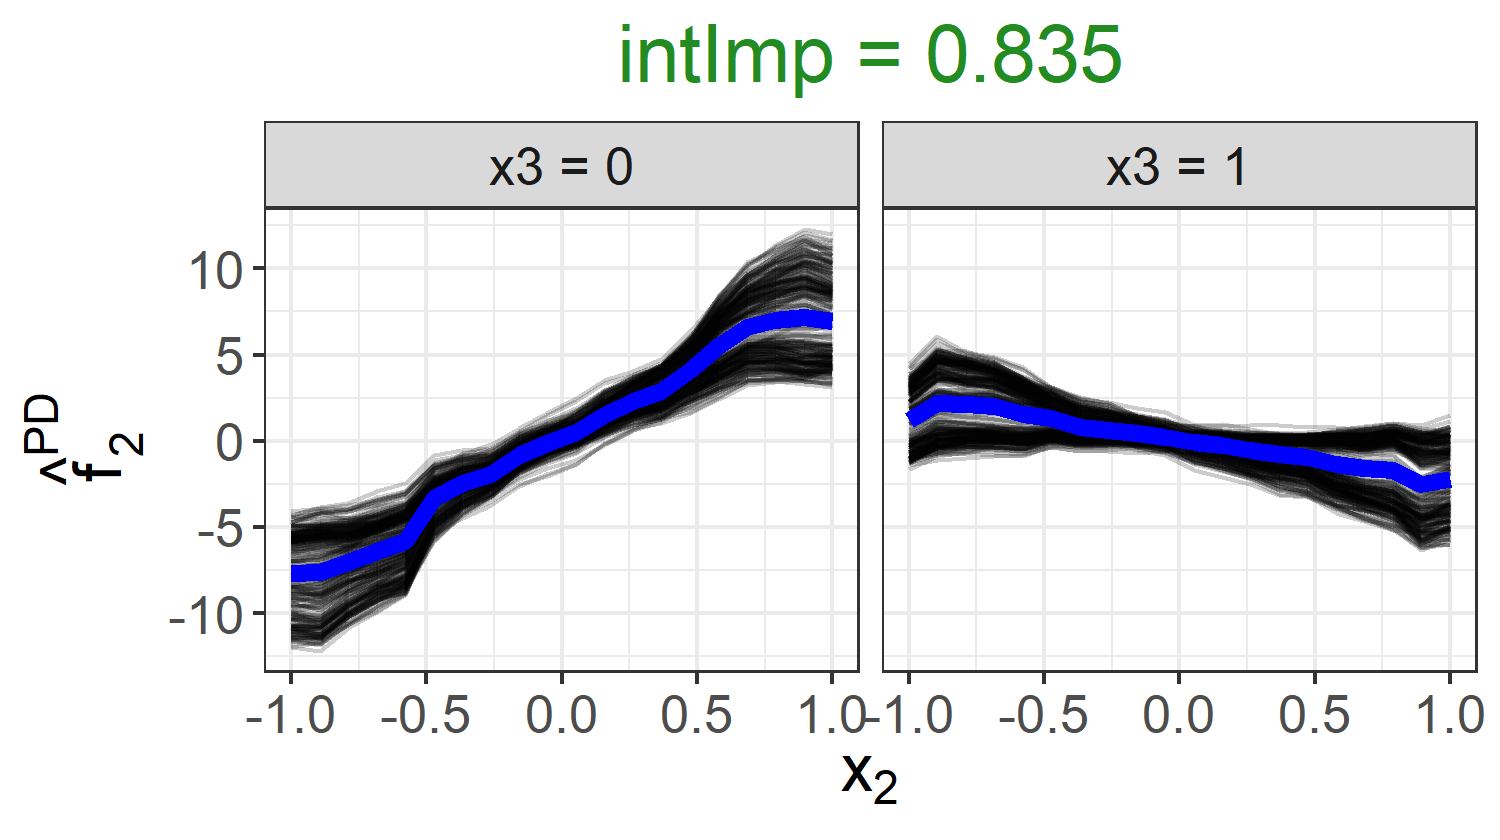
\includegraphics[width=0.6\textwidth, trim = 0 0 0 25, clip]{figure/sim1_dt_split1.png}
      }
      %}
}
\only<3->{
      \scalebox{1}{
      \hspace{15pt} 
      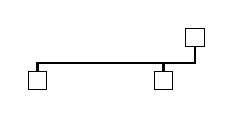
\begin{tikzpicture}
      \usetikzlibrary{arrows}
        \usetikzlibrary{shapes}
         \tikzset{treenode/.style={draw}}
         \tikzset{line/.style={draw, thick}}
        \node [treenode](a0) {} ; [below=1pt,at=(4,0)]  {};
         \node [treenode, below=0.3cm, at=(a0.south), xshift=-2.0cm]  (a1) {};
         \node [treenode, below=0.3cm, at=(a0.south), xshift=-0.4cm]  (a2) {};
         \path [line] (a0.south) -- + (0,-0.2cm) -| (a1.north) node [midway, above] {};
         \path [line] (a0.south) -- +(0,-0.2cm) -|  (a2.north) node [midway, above] {};
      \end{tikzpicture}
      \hspace{35pt}
      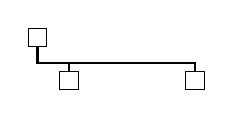
\begin{tikzpicture}
      \usetikzlibrary{arrows}
        \usetikzlibrary{shapes}
         \tikzset{treenode/.style={draw}}
         \tikzset{line/.style={draw, thick}}
        \node [treenode] (a01) {};[below=5pt,at=(node1.south) , xshift=3.5cm]
         \node [treenode, below=0.3cm, at=(a01.south), xshift=0.4cm]  (a1) {};
         \node [treenode, below=0.3cm, at=(a01.south), xshift=2.0cm]  (a2) {};
         \path [line] (a01.south) -- + (0,-0.2cm) -| (a1.north) node [midway, above] {};
         \path [line] (a01.south) -- +(0,-0.2cm) -|  (a2.north) node [midway, above] {};
      \end{tikzpicture}
      }
    %\fcolorbox{YellowGreen}{white}{
    YG{
    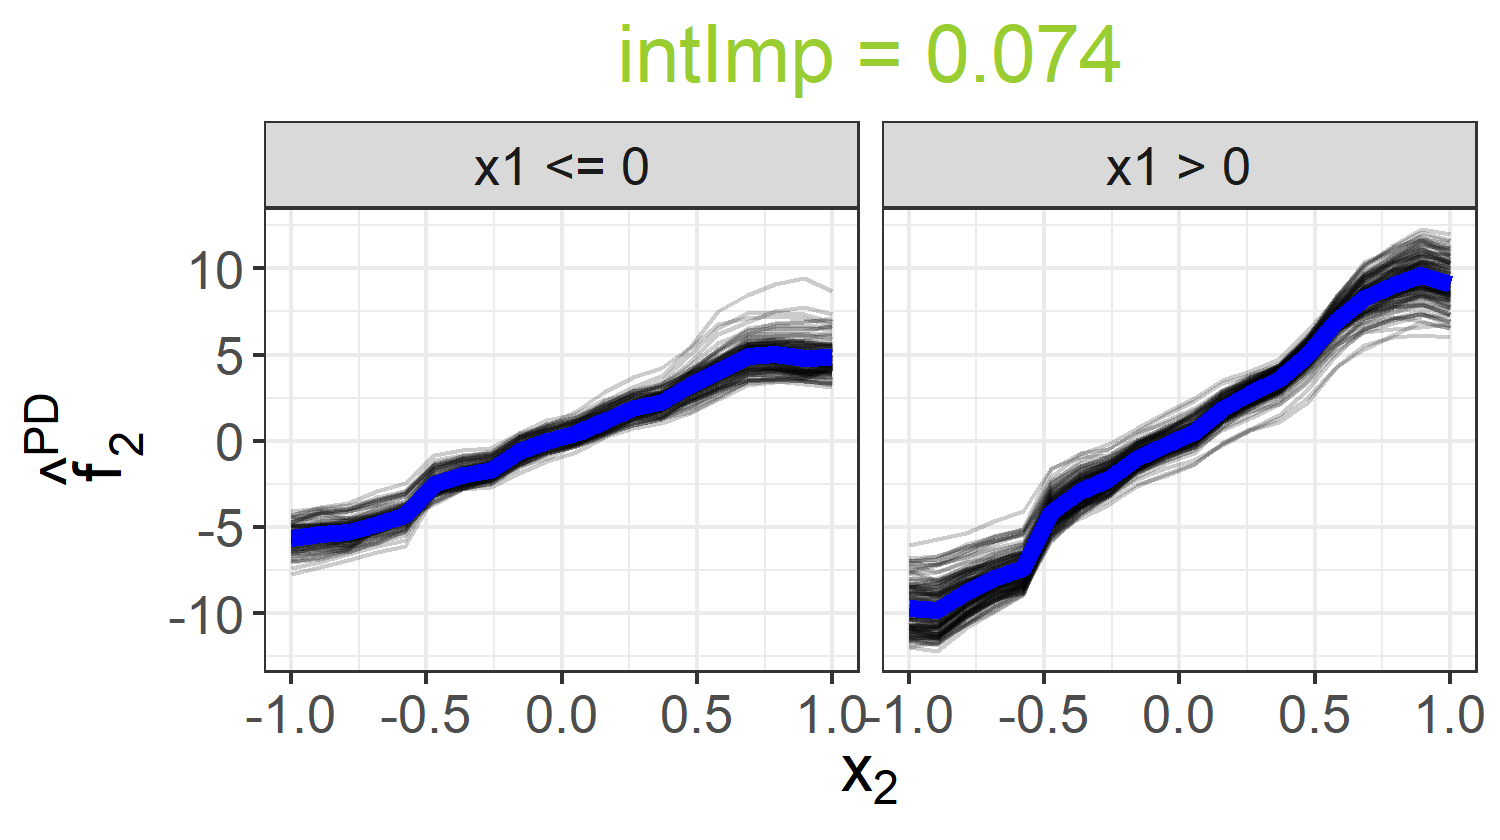
\includegraphics[width=0.52\textwidth, trim = 0 0 0 25, clip]{figure/sim1_dt_split2_1.png}
    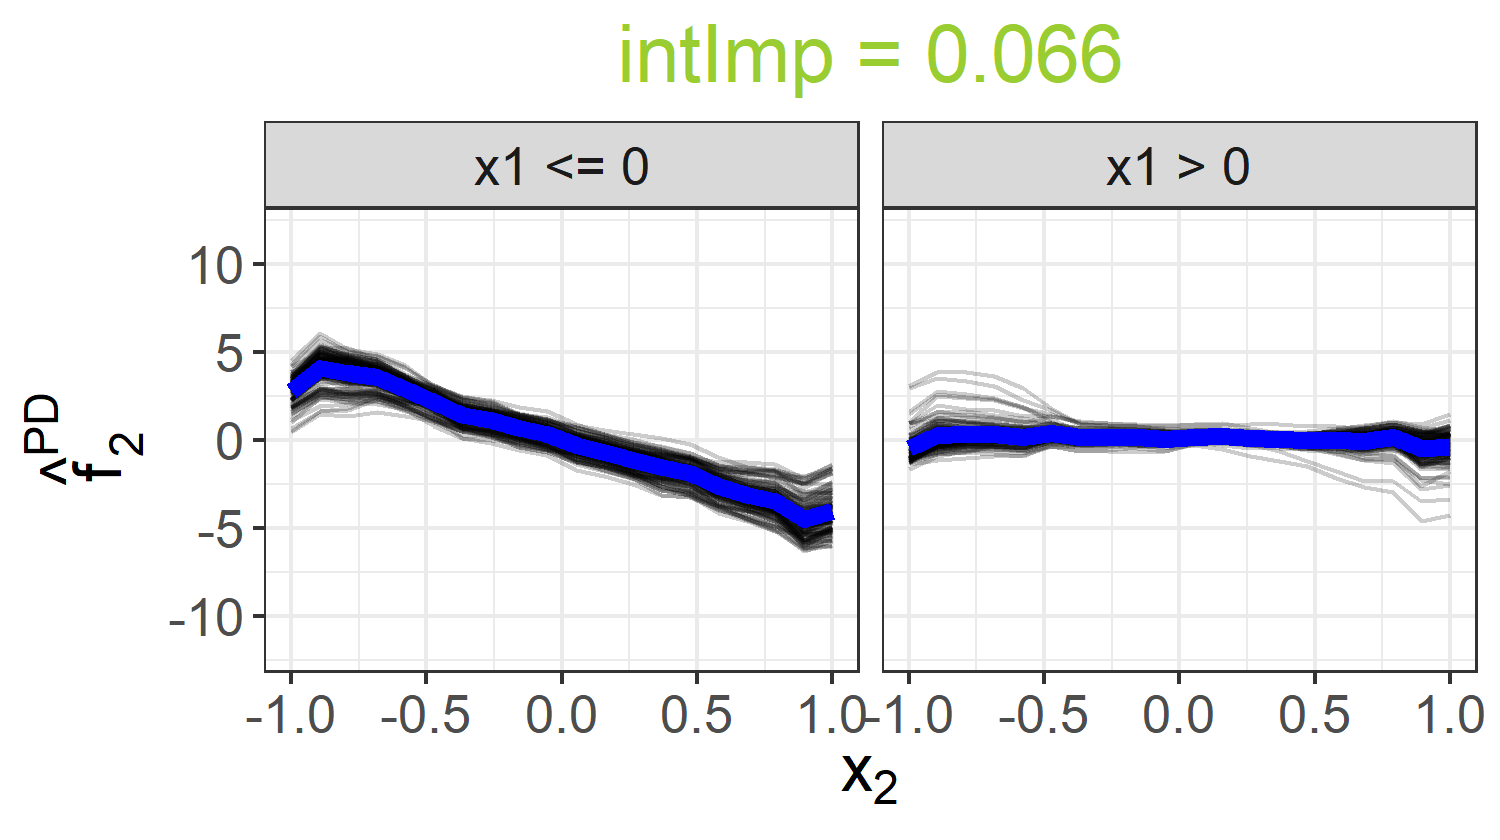
\includegraphics[width=0.46\textwidth, trim = 40 0 0 25, clip]{figure/sim1_dt_split2_2.png}
    }
    %\vspace{.2in}
    %\caption{ICE curves for $\xv_2$ are grouped by REPID and REPs (blue) are illustrated. %The first split divides the ICE curves depending on $x_3$. The second level divides the ICE curves of each child node again into two sub-regions with respect to $x_1$.
    %}
    %\label{fig:sim1_dt}
     %\end{minipage} 

     \begin{columns}[T, totalwidth = \linewidth]
     %\footnotesize
            \begin{column}{0.1\linewidth}
            \centering
             $\hat{f}_2^{PD}(X_2)$ %, X_1 > 0 \land X_3 = 0\)\\
         \end{column}
         \begin{column}{0.18\linewidth}
         \centering
             $\approx 8X_2$ %, X_1 > 0 \land X_3 = 0\)\\
         \end{column}
        \begin{column}{0.2\linewidth}
\centering
            $\approx 16X_2$ %, X_1 \leq 0 \land X_3 = 0\)
         \end{column}
        \begin{column}{0.2\linewidth}
        \centering
            $ \approx -8X_2$ %, X_1 \leq 0 \land X_3 \neq 0\)
         \end{column}        
         \begin{column}{0.2\linewidth}
         \centering
             $\approx 0$%, X_1 > 0 \land X_3 \neq 0\)\\
         \end{column}
     \end{columns}
     \medskip
     $\Rightarrow$ Additive decomposition of global feature effect
     %$f_2(X_2) \approx \sum_{i: \textit{terminal node indices}} g_i(X_2) \mathbbm{1}_{(X \in \mathcal{N}_i)}$
}


    \end{column}

\end{columns}

% \begin{minipage}[htb]{0.48\linewidth}
% \begin{itemize}

% \item \textbf{Problem:} PD plot (average of ICE) misleading

% \item \textbf{Idea:} Find regions where ICE curves are similar in their shape\\
% $\leadsto$ These regions have little interactions 

%     %\item<1-2> Grouping homogeneous ICE curves reduces individual interaction effects
%     %\item<2> REP = group marginal effect for feature of interest $x_j$ in specific region
  
% \end{itemize}
% \end{minipage}
% \only<1>{
% \begin{minipage}[htb]{0.5\linewidth}
%     \centering
%      %\begin{minipage}[t]{.5\textwidth}
%       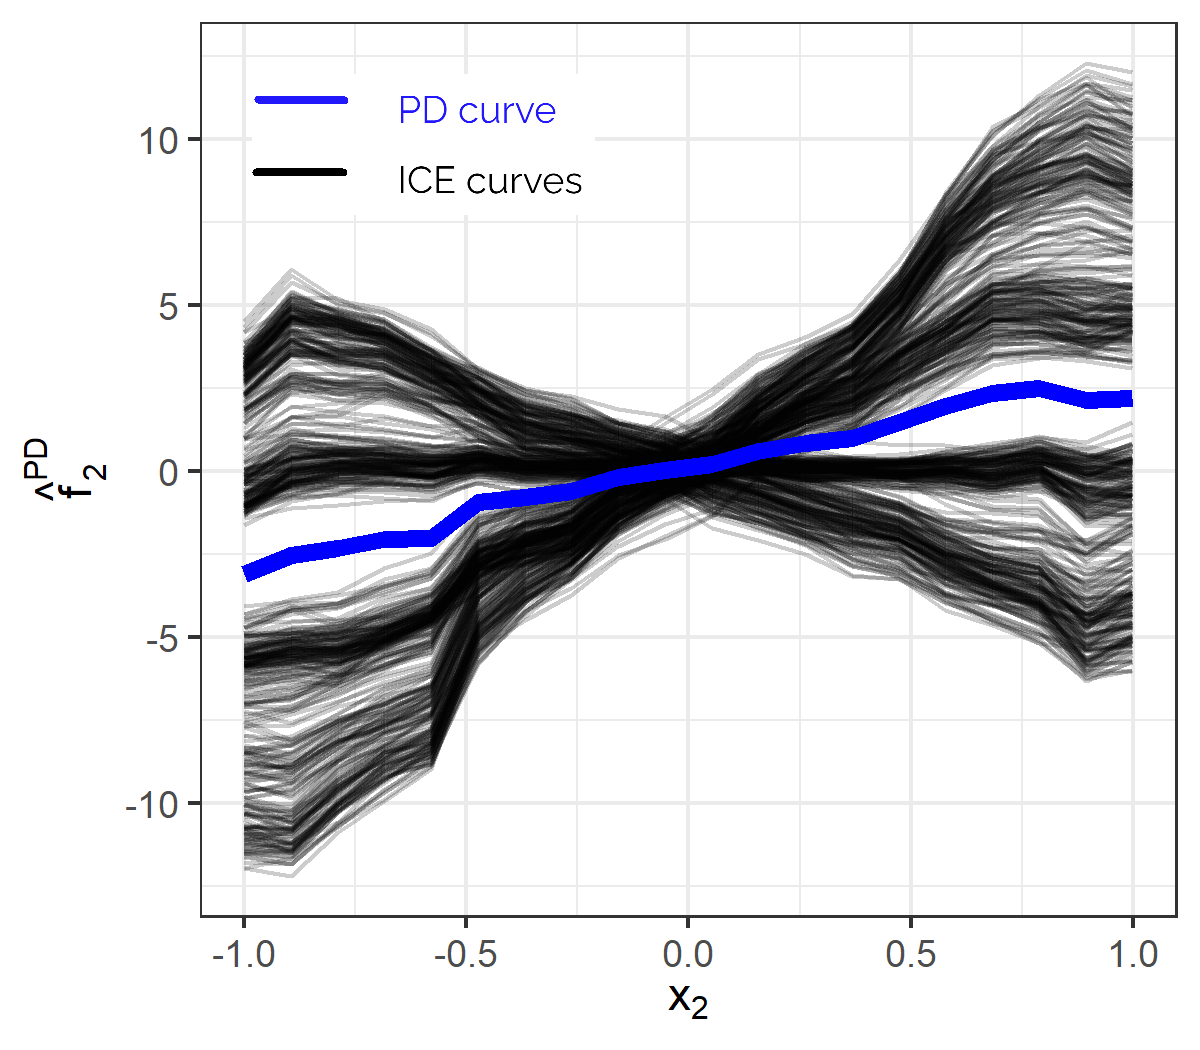
\includegraphics[width=0.9\textwidth]{figure/sim1_allcurves.png}
     
% \end{minipage}
% }
% \only<2>{
% \begin{minipage}[htb]{0.47\linewidth}
%     \centering
%      %\begin{minipage}[t]{.5\textwidth}
%       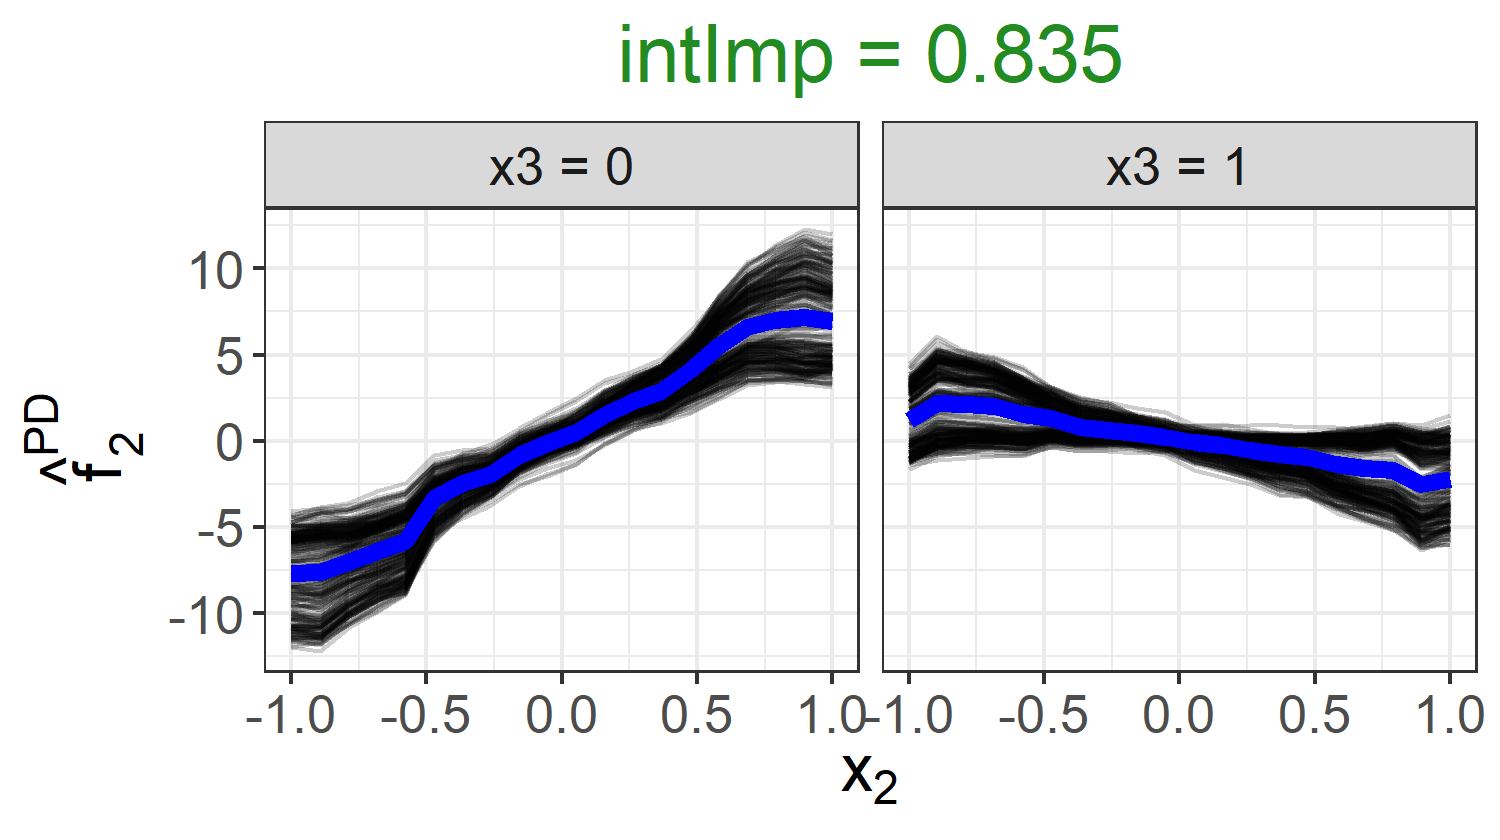
\includegraphics[width=0.49\textwidth]{figure/sim1_dt_split1.png}
%       \scalebox{1}{
%       \hspace{15pt} 
%       \begin{tikzpicture}
%       \usetikzlibrary{arrows}
%         \usetikzlibrary{shapes}
%          \tikzset{treenode/.style={draw}}
%          \tikzset{line/.style={draw, thick}}
%         \node [treenode](a0) {} ; [below=1pt,at=(4,0)]  {};
%          \node [treenode, below=0.3cm, at=(a0.south), xshift=-2.0cm]  (a1) {};
%          \node [treenode, below=0.3cm, at=(a0.south), xshift=-0.4cm]  (a2) {};
%          \path [line] (a0.south) -- + (0,-0.2cm) -| (a1.north) node [midway, above] {};
%          \path [line] (a0.south) -- +(0,-0.2cm) -|  (a2.north) node [midway, above] {};
%       \end{tikzpicture}
%       \hspace{35pt}
%       \begin{tikzpicture}
%       \usetikzlibrary{arrows}
%         \usetikzlibrary{shapes}
%          \tikzset{treenode/.style={draw}}
%          \tikzset{line/.style={draw, thick}}
%         \node [treenode] (a01) {};[below=5pt,at=(node1.south) , xshift=3.5cm]
%          \node [treenode, below=0.3cm, at=(a01.south), xshift=0.4cm]  (a1) {};
%          \node [treenode, below=0.3cm, at=(a01.south), xshift=2.0cm]  (a2) {};
%          \path [line] (a01.south) -- + (0,-0.2cm) -| (a1.north) node [midway, above] {};
%          \path [line] (a01.south) -- +(0,-0.2cm) -|  (a2.north) node [midway, above] {};
%       \end{tikzpicture}
%       }
%     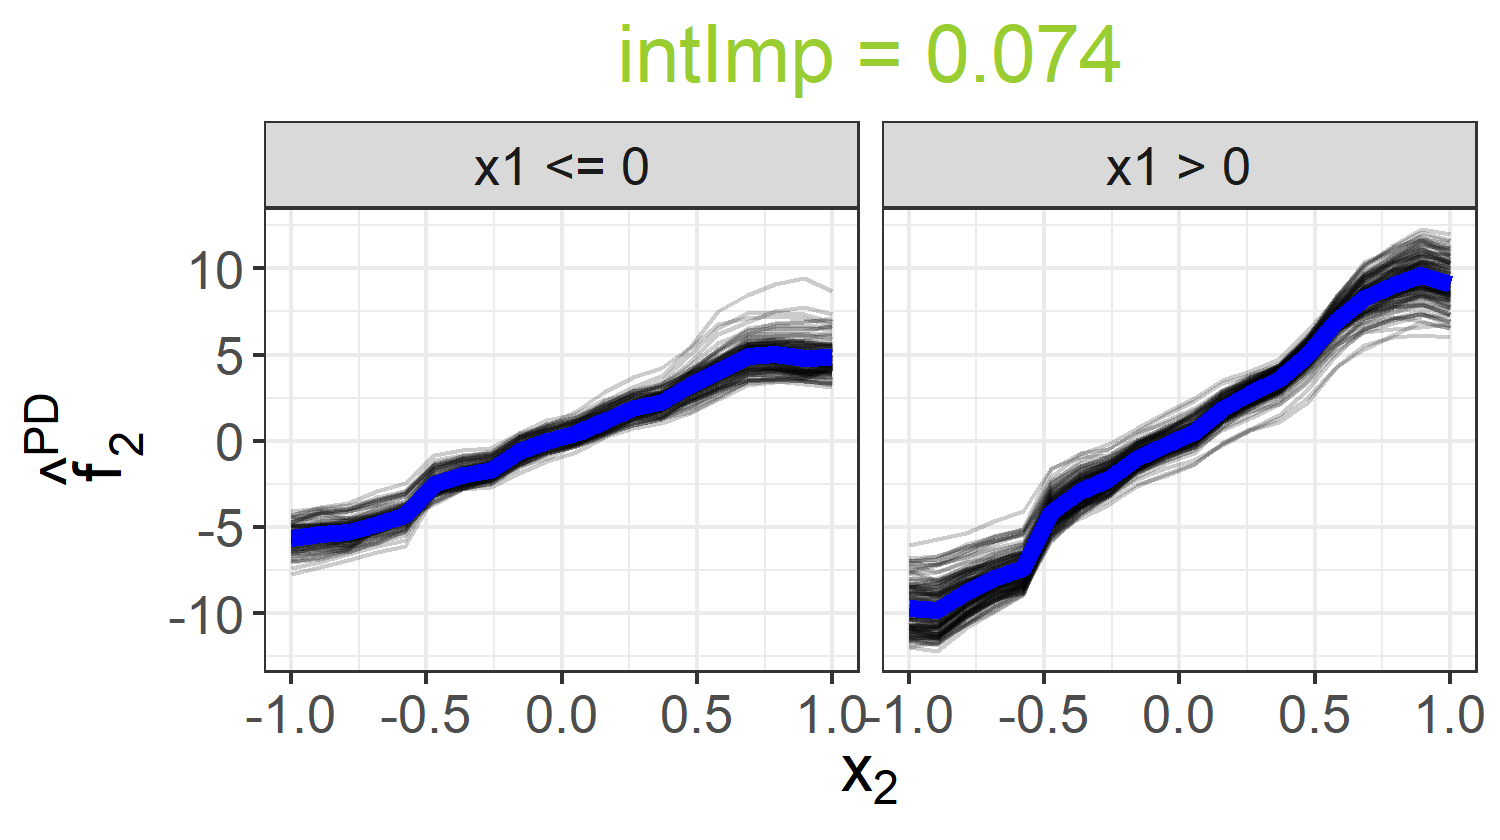
\includegraphics[width=0.49\textwidth]{figure/sim1_dt_split2_1.png}
%     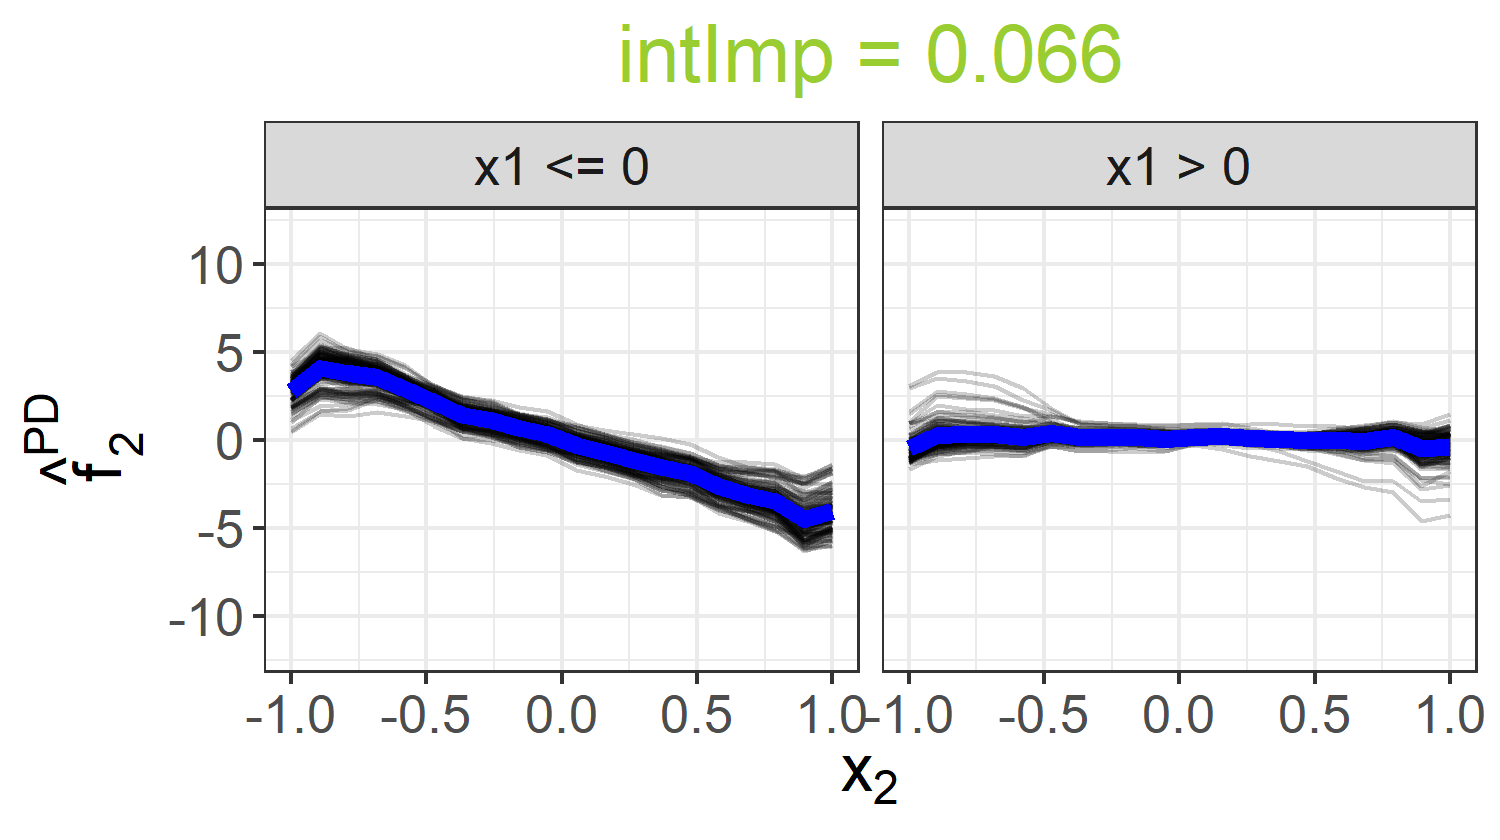
\includegraphics[width=0.49\textwidth]{figure/sim1_dt_split2_2.png}
%     \vspace{.2in}
%     %\caption{ICE curves for $\xv_2$ are grouped by REPID and REPs (blue) are illustrated. %The first split divides the ICE curves depending on $x_3$. The second level divides the ICE curves of each child node again into two sub-regions with respect to $x_1$.
%     %}
%     \label{fig:sim1_dt}
%      %\end{minipage} 
%\end{minipage}
%}


%\footnote[frame]{\textbf{AISTATS 2022:} \textit{REPID - Regional Effect Plots with implicit Interaction Detection}}
\end{frame}

\endlecture
\end{document}
